%%%%%%%%%%%%%%%%%%%%%%%%%%%%%%%%%%%%%%%%%%%%%%%%%%%%%%%%%%%%%%%%%%%%%%%%%%%
%% This file is part of the book
%%
%% Algorithmic Graph Theory
%% http://code.google.com/p/graph-theory-algorithms-book/
%%
%% Copyright (C) 2009--2011 Minh Van Nguyen <nguyenminh2@gmail.com>
%%
%% See the file COPYING for copying conditions.
%%%%%%%%%%%%%%%%%%%%%%%%%%%%%%%%%%%%%%%%%%%%%%%%%%%%%%%%%%%%%%%%%%%%%%%%%%%

\documentclass{article}

\usepackage{subfigure}
\usepackage{tikz}
\usetikzlibrary{external}
\usetikzlibrary{trees}
\tikzexternalize{binary-search-tree-insert}

\begin{document}

\begin{figure}
\subfigure[]{
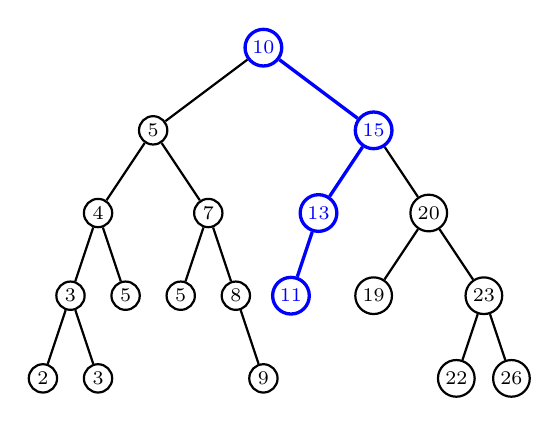
\begin{tikzpicture}
[-,thick,%
  every node/.style={shape=circle,inner sep=1.5pt,draw,thick},%
  scale=0.7]
\scriptsize
\node[blue,very thick] {$10$}
  [sibling distance=4cm]
  child {node {$5$}
    [sibling distance=2cm]
    child {node {$4$}
      [sibling distance=1cm]
      child {node {$3$}
        child {node {$2$}}
        child {node {$3$}}
      }
      child {node {$5$}}
    }
    child {node {$7$}
      [sibling distance=1cm]
      child {node {$5$}}
      child {node {$8$}
        child[missing]
        child {node {$9$}}
      }
    }
  }
  child[blue,very thick] {node[blue,very thick] {$15$}
    [sibling distance=2cm]
    child {node[blue,very thick] {$13$}
      [sibling distance=1cm]
      child {node[blue,very thick] {$11$}}
      child[missing]
    }
    child[black,thick] {node {$20$}
      child {node {$19$}}
      child {node {$23$}
        [sibling distance=1cm]
        child {node {$22$}}
        child {node {$26$}}
      }
    }
  };
\end{tikzpicture}
}
%%
%%
\qquad
\subfigure[]{
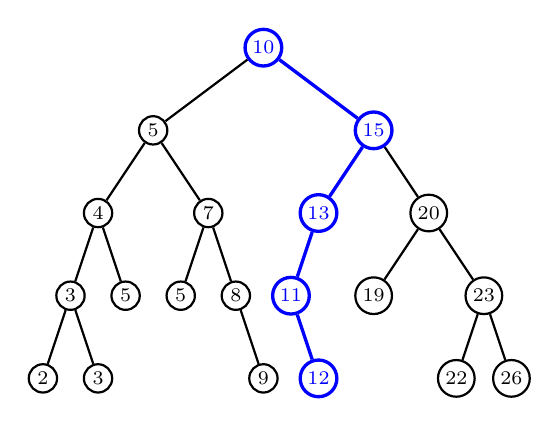
\begin{tikzpicture}
[-,thick,%
  every node/.style={shape=circle,inner sep=1.5pt,draw,thick},%
  scale=0.7]
\scriptsize
\node[blue,very thick] {$10$}
  [sibling distance=4cm]
  child {node {$5$}
    [sibling distance=2cm]
    child {node {$4$}
      [sibling distance=1cm]
      child {node {$3$}
        child {node {$2$}}
        child {node {$3$}}
      }
      child {node {$5$}}
    }
    child {node {$7$}
      [sibling distance=1cm]
      child {node {$5$}}
      child[black,thick] {node {$8$}
        child[missing]
        child {node {$9$}}
      }
    }
  }
  child[blue,very thick] {node[blue,very thick] {$15$}
    [sibling distance=2cm]
    child {node[blue,very thick] {$13$}
      [sibling distance=1cm]
      child {node[blue,very thick] {$11$}
        child[missing]
        child {node[blue,very thick] {$12$}}
      }
      child[missing]
    }
    child[black,thick] {node {$20$}
      child {node {$19$}}
      child {node {$23$}
        [sibling distance=1cm]
        child {node {$22$}}
        child {node {$26$}}
      }
    }
  };
\end{tikzpicture}
}
\end{figure}

\end{document}
